%------------------------------------------------
% Quick reference.
%------------------------------------------------
%
% Для вставки картинок:
%
%--------         Комманда
%
%\begin{figure}[H]
%	\includegraphics{img_name}
%	\caption{some caption}
%	\label{some_pic}
%\end{figure}
%
%--------        Переменные
%
% img_name     <- Название картинки в папке img.
% some_caption <- подпись картинки.
% label        <- лейбл нужен для ссылок на картинку.
% H            <- расположение картинки на странице.
%
%--------         Пример
%
%\begin{figure}[H]
%	\includegraphics{pic1.jpg}
%	\caption{График зависимости какой-то хуйни}
%	\label{grapics1}
%\end{figure}
%
%------------------------------------------------
%
% Для референса по лейблу:
%
%--------         Комманда
%
% Для ссылки используется \eqref{ref}.
%
%--------        Переменные
%
% ref          <- указанный лейбл в директиве \label{ref}
%                 Ссылку можно сделать на любой объект имеющий \label{•}
%
%--------         Пример
%
% \eqref{graphics1}
%
%------------------------------------------------
%
% Для листинга кода:
%
%--------         Комманда
%
% \lstinputlisting[language=lang,mathescape=true]{src}
%--------        Переменные
%
% lang         <- язык на котором написан исходный код, например "python" или "C++".
% mathescape   <- если в исходниках есть формулы LaTeX, то они будут представлены как формулы.
% src          <- путь до файла исходников.
%
%--------         Пример
%
% \lstinputlisting[language=C++,mathescape=false]{./src/bullshit.cpp}
%
%------------------------------------------------
%
% Для вставки таблиц:
%
%--------
%\begin{table}[H]
%	\centering
%	\caption{ capt }
%	\begin{tabularx}{0.9\textwidth}{ | Y | Y | }
%		\hline
%		lines
%	\end{tabularx}
%	\label{tab1}
%\end{table}
%--------
% caption      <- Подпись таблицы.
% tab1         <- лейбл нужный для ссылки на таблицу.
% | Y | Y |    <- количество и формат столбцов.
% Y            <- Тип столбца.
%                 В данном случае определены кастомные столбцы Y (Спасибо Максиму Наумову)
% |            <- обозначает границы столбца.
%                 То есть, если будет указано |Y Y|, то столбцы внутри строк разделены не будут.
% H            <- То же самое, что и у картинок.
% lines        <- непосредственно элементы таблицы.
%                 Разделяются знаком "&", оканчивать каждую строку лучше \\ \hline
%
%--------         Пример
%\begin{table}[H]
%	\centering
%	\caption{ capt }
%	\begin{tabularx}{0.9\textwidth}{ | Y | Y | }
%		\hline
%		str1 & str2 \\ \hline
%		str1 & str2 \\ \hline
%		str1 & str2 \\ \hline
%		str1 & str2 \\ \hline
%		str1 & str2 \\ \hline
%	\end{tabularx}
%	\label{tab1}
%\end{table}
%------------------------------------------------

\documentclass[14pt, a4paper, fleqn]{extarticle}

\makeatletter
\renewcommand*\l@section{\@dottedtocline{1}{1.5em}{2.3em}}



%\includegraphics{universe}

\usepackage[utf8]{inputenc}
\usepackage[T2A]{fontenc}
\usepackage[russian]{babel} % указывает язык документа
\usepackage[left=3cm,right=2cm,top=2cm,bottom=2cm,bindingoffset=0cm]{geometry}
\usepackage{lastpage}
\usepackage{fancyhdr}
\usepackage{titlesec}
\usepackage{graphicx} % для вставки картинок
\usepackage[intlimits]{mathtools} % математические дополнения
\usepackage{amssymb}
\usepackage[tableposition=top]{caption}
\usepackage{subcaption}
\usepackage{indentfirst}
\usepackage{pythonhighlight}
\usepackage{listings}
\usepackage{tabularx}
\usepackage{tabulary}
\usepackage{multirow}
\usepackage{float}
\usepackage[figure,table]{totalcount}
\usepackage{diagbox}
\usepackage[german=guillemets]{csquotes}
\usepackage{fontspec}
\usepackage{enumitem}
%\usepackage{mathptmx}% http://ctan.org/pkg/mathptmx
%\usepackage{showframe}
\usepackage{hyperref}

\setlength{\parindent}{1.2cm}

\setlength{\mathindent}{1.2cm}

\defaultfontfeatures{Ligatures={TeX},Renderer=Basic}
\setmainfont[Ligatures={TeX,Historic}]{Times New Roman}

%\setlist[enumerate]{itemindent=\dimexpr\labelwidth+\labelsep\relax,leftmargin=0pt}

%\setlength{\section*}{0.5cm}
%\usepackage{minted}
%\usepackage{fancyvrb}
%\usepackage{newtxtext}

%\titleformat{\section}[hang]{\bfseries\LARGE\centering}{}{1em}{}

%\setlist[enumerate]{itemindent=\dimexpr\labelwidth+\labelsep\relax,leftmargin=0pt}
\setlist[enumerate,itemize]{leftmargin=0pt,itemindent=1.7cm}
\titlespacing*{\section}{0.6cm}{1ex}{1em}
\titleformat{\section}{\large\bfseries\centering}{\thesection}{0.5em}{\MakeUppercase}
\titleformat{\subsection}[block]{\bfseries\hspace{1em}}{\thesubsection}{0.5em}{}
%\setlength{\subsection*}{1.5cm}
%\setlength{\parindent}{4em}

%\setlength{\parindent}{1.5cm}

\captionsetup[figure]{labelfont={it},textfont={it},name={Рисунок},labelsep=endash, skip=5pt}
\captionsetup[table]{labelfont={it},textfont={it},name={Таблица},labelsep=endash,singlelinecheck=false, skip=5pt, margin=1cm}


%\renewcommand{\baselinestretch}{1.5}
\linespread{1.5} % полуторный интервал
\frenchspacing
\graphicspath{ {images/} }


  %-------------------------------------------
  % Переменные
  %-------------------------------------------

  \newcommand{\firstAuthorSurName}{Кирилин} 					                           % Фамилия автора.
  \newcommand{\firstAuthorInitials}{ П. Н.} 					                           % Фамилия автора.
  \newcommand{\leftcolon}{Технологии сетевого программирования}
  \newcommand{\secondAuthorSurName}{Наумов} 					                           % Фамилия автора.
  \newcommand{\secondAuthorInitials}{ М. Е.} 					                           % Фамилия автора.
  \newcommand{\teacherName}{Белоусов А. А.}				                               % Имя преподавателя.
  \newcommand{\variantNumber}{33} 							                           % Номер варианта.
  \newcommand{\groupNumber}{6409-010302D} 				                               % Номер группы.
  \newcommand{\subjectTitle}{Курсовой проект по дисциплине}                                  % Название предмета.
  \newcommand{\taskTitle}{Технологии сетевого программирования}    % Название работы.
  \newcommand{\theme}{Сервис предзаказа еды} 		  % Название работы.
  
  %-------------------------------------------
  % Ссылки в оглавлении
  %-------------------------------------------

\hypersetup{
    colorlinks,
    citecolor=black,
    filecolor=black,
    linkcolor=black,
    urlcolor=black
}

%-------------------------------------------
% Стиль футеров и хедеров
%-------------------------------------------

\pagestyle{fancy}
\fancyhead[L, R]{}
\fancyfoot[L]{}
\fancyfoot[R]{}
\renewcommand{\footrulewidth}{0pt}
\renewcommand{\headrulewidth}{0pt}

%\renewcommand\subsectionfont{\normalfont\normalsize\bfseries}

\def\l@subsection{\@dottedtocline{2}{3.8em}{3.2em}}
\setcounter{tocdepth}{2}
% Для листинга

\lstset{
basicstyle=\footnotesize\ttfamily,
columns=fullflexible,
keywordstyle=\color{blue},
%frame=single,
breaklines=true,
numberstyle=\tiny\color{mygray},
postbreak=\mbox{\textcolor{red}{$\hookrightarrow$}\space},
showstringspaces=false,
}

\newcolumntype{Y}{>{\centering\arraybackslash}X}

\begin{document}
\pagenumbering{Alph}

\begin{titlepage}
							
	\center
							
	%------------------------------------------------
	%	Заголовки
	%------------------------------------------------
							
	\textsc{Министерство науки и высшего образования Российской Федерации}\\[-0.15cm]
	\textsc{Федеральное государственное автономное образовательное учреждение \\[-0.15cm] высшего образования}\\[-0.15cm] 
	\textsc{«Самарский национальный исследовательский университет \\[-0.15cm] имени академика С.П.Королёва»}\\[0.25cm]
	\textsc{Факультет информатики}\\[0.1cm]
	\textsc{Кафедра технической кибернетики}\\[0.5cm]
						
	%------------------------------------------------
	%	Название работы
	%------------------------------------------------
							
	\vfill\vfill
						    
							
	{\subjectTitle}\\[0.3cm]
	
	{\enquote{\taskTitle}}\\[0.5cm]
						  
    {\textbf{\theme}}\\[0.5cm]

    \vfill\vfill\vfill
							
	\begin{minipage}{1\textwidth}
		\begin{center}
			\begin{tabularx}{\textwidth}{X l}
				Выполнили студенты:        & \firstAuthorSurName \firstAuthorInitials \\
				                           & \secondAuthorSurName \secondAuthorInitials \\
				Группа:                    & 6409                     		           \\
				Проверил:                  & \teacherName         		                \\
			\end{tabularx}
		\end{center}
	\end{minipage}
							
						
	%------------------------------------------------
	%	Дата
	%------------------------------------------------
							
	\vfill\vfill\vfill
					
	{\centering Самара \the\year}
							
							
\end{titlepage}
\pagenumbering{arabic}

\setcounter{page}{2}

%------------------------------------------------
% Реферат
%------------------------------------------------
\phantomsection
\section*{РЕФЕРАТ}
{
	Отчёт:
	\pageref{LastPage} страницы,
	\totalfigures\ рисунков,
	\totaltables\ таблицы,
	10 источников,
	1 приложение.\\

	\textit{ТЕХНОЛОГИИ СЕТЕВОГО ПРОГРАММИРОВАНИЯ, RUBY ON RAILS, VUE, АРХИТЕКТУРА, ВЕБ-ИНТЕРФЕЙС, POSTGRESQL}\\

	Цель работы - создание трехуровневого приложения, работающего с базой данных, описывающей работу \enquote{Сервиса предзаказа еды}.
}
\newpage

\newpage
\tableofcontents


%------------------------------------------------
% Введение
%------------------------------------------------
\newpage
\phantomsection
\addcontentsline{toc}{section}{Введение}
\section*{Введение}
{
 Данное приложение позволит вам совершать предзаказ и получать еду к назначенному времени.

Пользователю предоставляется выбор ресторана, где он может совершить заказ. В каждом ресторане имеется меню товаров, доступных для заказа. После составления заказа, пользователю предлагается сообщается о времени, к которому заказ должен быть приготовлен.

Сервис \enquote{feedEm}не имеет очередей ожидания. Всё, что понадобится для заказа - соединение с сетью интернет.

Заказ пользователя готовится к назначенному времени и вместо ожидания в очереди нужно только забрать заказ.

 Обычным пользователям системы предоставляются следующие возможности:
 \begin{enumerate}
     \item {Регистрация аккаунта;}
     \item {Поиск интересующего товара по названию и описанию;}
     \item {Добавление понравившихся товаров в корзину;}
 \end{enumerate}
Зарегистрированные пользователи имеют права на:
 \begin{enumerate}
     \item{Добавление кредитных кат, с помощью которых производится оплата;}
     \item{Оплата товаров, находящихся в корзине;}
     \item{Отменить заказ;}
     \item{Поставить оценку продавцу.}
 \end{enumerate}
Продавцы зарегистрированные в системе \enquote{feedEm} могут:
 \begin{enumerate}
     \item{Редактировать меню товаров, предоставляемое пользователям;}
     \item{Отменить заказ;}
     \item{Сообщить пользователю о готовности заказа;}
     \item{Запросить новый токен для аутентификации.}
 \end{enumerate}
Администраторы имеют следующие возможности:
 \begin{enumerate}
     \item {Изменять аккаунты клиентов;}
     \item {Изменять аккаунты продавцов;}
     \item {Изменять аккаунты администраторов;}
     \item {Изменять товары;}
     \item {Изменять совершенные заказы;}
 \end{enumerate}
}
\newpage


%------------------------------------------------
% Начало основной части
%------------------------------------------------
\titleformat{\section}{\large\bfseries}{\thesection}{0.5em}{}
\titlespacing*{\section}{1.1cm}{1ex}{1em}
\titlespacing*{\subsection}{0.6cm}{1ex}{1em}
\section{Обоснование выбора технологий}
{
    Разработка приложения велась на языке Ruby[\ref{src_ruby}], с использованием фреймворка Rails[\ref{src_rails}] с использованием JavaScript фреймворка Vue[\ref{src_vue}]. Выбор обусловлен тем, что разработка приложений с использованием фреймворка \enquote{Ruby on rails} существенно ускоряет и упрощает разработку серверной части приложения и настройку окружения для разрабатываемого приложения, в которое входит взаимодействие с системами управления базами данных, а также всё необходимое для разработки клиентской части приложения.
}
\newpage

\section{Сценарии использованая приложения}
{
\subsection{Уменьшить время ожидания для покупателей}
{
Данное приложение позволит вам совершать предзаказ и получать еду к назначенному времени.

Пользователю предоставляется выбор ресторана, где он может совершить заказ. В каждом ресторане имеется меню возможных товаров. После составления заказа, пользователю показывается время, к которому заказ должен быть приготовлен.

Сервис feeEm не имеет очередей ожидания. Всё, что понадобится для заказа - соединение с сетью интернет.

Заказ пользователя готовится к назначенному времени и вместо ожидания в очереди нужно только забрать заказ.

\begin{enumerate}
  \item {
    Покупатель может просматривать каталоги ресторанов.

    Для просмотра меню ресторана нужно выполнить следующую последовательность действий:

      \begin{enumerate}[label*=\arabic*.]
      \item Зайти на сайт;
      \item Зарегестрироваться (Если нужно);
      \item Пройти авторизацию;
      \item Осуществить поиск интересующего ресторана (Поиск осуществляется по описанию, названию, по товарам);
      \item Выбрать ресторан.
      \end{enumerate}

    После выполненных действий пользователю будет доступно меню выбранного ресторана.
  }

  \item {
    Покупатель может осуществить заказ онлайн.

    Для совершения заказа нужно выполнить следующую последовательность действий:

    \begin{enumerate}[label*=\arabic*.]
      \item Открыть меню интересующего ресторана;
      \item Добавить интересующие пункты меню в корзину;
      \item Добавить кредитную карту (Если нужно);
      \item Проверить примерное время заказа (Если устраивает, то продолжить);
      \item Заказать и оплатить заказ.
    \end{enumerate}
  }

  \item {
    Рейтинговая система для выбора лучшего магазина.

    Также, пользователи могут поставить оценку ресторану, что поможет другим пользователям выбрать продавца с наилучшим сервисом. Чтобы это сделать нужно:

    \begin{enumerate}[label*=\arabic*.]
      \item Открыть страницу ресторана;
      \item Поставить оценку (Нравится или не нравится).
    \end{enumerate}
  }
\end{enumerate}
}

\subsection{Увеличение дохода ресторана}
{
  FeedEm создан не для доставки, а для предзаказов. Цель продавцов - подготовка еды к нужному для клинтов времени. Покупатели сам придут, чтобы получить заказ.

  \begin{enumerate}
    \item {
      Составление меню для продажи онлайн.

      Для сосавления меню нужно выполнить следующие действия:

      \begin{enumerate}[label*=\arabic*.]
        \item Открыть страницу упраления рестораном.
        \item Открыть страницу редактирования меню.
        \item Добавить/отредактировать/удалить товары.
      \end{enumerate}
    }
    \item {
      Прием заказов онлайн.

      Для приема доступных заказов:

      \begin{enumerate}[label*=\arabic*.]
        \item Открыть страницу упраления рестораном.
        \item Открыть вкладку заказов.
        \item Принять/отредактировать примерное время/отклонить заказы.
      \end{enumerate}
    }
    \item {
      Просмотр рейтинга ресторанов.

      Просмотр наиболее популярных ресторанов может помочь узнать, что сейчас интересно покупателям.

      Для просмотра рейтинга рестораноа:

      \begin{enumerate}[label*=\arabic*.]
        \item Открыть страницу выбора ресторана. На данной странице представлены рестораны, отсортированные по рейтингу.
      \end{enumerate}

      Изменение рейтинга ресторана доступно только для авторизированных покупателей.
    }
  \end{enumerate}
}
}
\newpage

\section{Структура базы данных}
{
    \subsection{Схемы базы данных}
    На рисунках \ref{logic_db} и \ref{physical_db} изображены логическая и физическая схемы базы данных.
    \begin{figure}[H]
    \centering
    	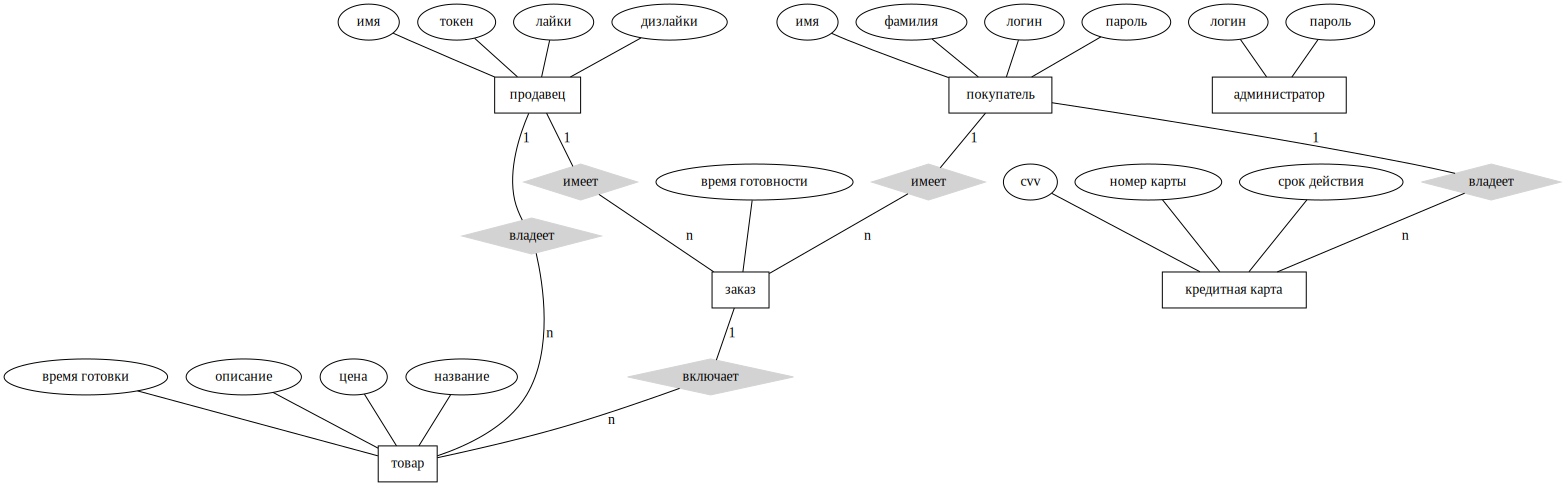
\includegraphics[width=\textwidth]{ER.png}
    	\caption{Логическая схема базы данных}
    	\label{logic_db}
    \end{figure}

    \begin{figure}[H]
    \centering
    	\includegraphics[width=\textwidth]{erd.png}
    	\caption{Физическая схема базы данных}
    	\label{physical_db}
    \end{figure}

    В приложении А представлены скрипты генерации и заполнения баз данных.

    \subsection{Описание сущностей}
    Краткое описание сущностей приведено в таблицах \ref{customers_table_desc}, \ref{sellers_table_desc}, \ref{admins_table_desc}, \ref{merch_table_desc}, \ref{order_table_desc}, \ref{card_table_desc}, \ref{order_item_desc}.

    \begin{table}[H]
    	\centering
    	\caption{Описание сущности \enquote{покупатель}}
    	\begin{tabularx}{0.9\textwidth}{ | Y | Y | Y |}
    		\hline
    		Таблица          &  Атрибут & Описание \\ \hline
    		customers        & \multicolumn{2}{c|}{Содержит информацию о покупателях.} \\ \hline
    		[Первичный ключ] & id       & Уникальный идентификатор покупателя. \\ \hline
    		                 & name     & Имя покупателя. \\ \hline
    		                 & surname  & Фамилия покупателя. \\ \hline
    		[Вторичный ключ] & email    & Электронная почта покупателя. \\ \hline
    		                 & password & Зашифрованный пароль покупателя. \\ \hline
    	\end{tabularx}
    	\label{customers_table_desc}
    \end{table}

    \begin{table}[H]
           	\centering
           	\caption{ Описание сущности \enquote{продавец} }
           	\begin{tabularx}{0.9\textwidth}{ | Y | Y | Y |}
           		\hline
    		Таблица          &  Атрибут & Описание \\ \hline
    		         sellers & \multicolumn{2}{c|}{Содержит информацию о продавцах.} \\ \hline
    		[Первичный ключ] & id       & Уникальный идентификатор продавца. \\ \hline
    		[Вторичный ключ] & token    & Зашифрованный пароль продавца. \\ \hline
    		                 & likes    & Количество положительных оценок. \\ \hline
    		                 & dislikes & Количество отрицательных оценок. \\ \hline           	\end{tabularx}
           	\label{sellers_table_desc}
           \end{table}

    \begin{table}[H]
       \centering
       \caption{Описание сущности \enquote{администратор}}
       \begin{tabularx}{0.9\textwidth}{ | Y | Y | Y | }
       	\hline
       	    		Таблица  &  Атрибут & Описание \\ \hline
    		          admins & \multicolumn{2}{c|}{Содержит информацию об администраторах.} \\ \hline
    		[Первичный ключ] & id       & Уникальный идентификатор администратора. \\ \hline
    		[Вторичный ключ] & email    & Электронная почта администратора. \\ \hline
    		                 & password & Зашифрованный пароль администратора. \\ \hline       \end{tabularx}
       \label{admins_table_desc}
    \end{table}

     \begin{table}[H]
       \centering
       \caption{Описание сущности \enquote{товар}}
       \begin{tabularx}{0.9\textwidth}{ | Y | Y | Y | }
       	\hline
       	    		Таблица  &  Атрибут & Описание \\ \hline
    		          merchandises      & \multicolumn{2}{c|}{Содержит информацию о товарах.} \\ \hline
    		[Первичный ключ] & id       & Уникальный идентификатор товара. \\ \hline
    		[Вторичный ключ] & seller\_id & Ключ продавца товара. \\ \hline
    		                 & name     & Название товара. \\ \hline
    		                 & description & Описание товара. \\ \hline
    		                 & cook\_time  & Время приготовления товара. \\ \hline
    		                 & price       & Цена товара.  \\ \hline
        \end{tabularx}
       \label{merch_table_desc}
    \end{table}

     \begin{table}[H]
       \centering
       \caption{Описание сущности \enquote{заказ}}
       \begin{tabularx}{0.9\textwidth}{ | Y | Y | Y | }
       	\hline
       	    		Таблица  &  Атрибут & Описание \\ \hline
    		          orders & \multicolumn{2}{c|}{Содержит информацию о заказах.} \\ \hline
    		[Первичный ключ] & id       & Уникальный идентификатор заказа. \\ \hline
    		                 & name     & Название зак. \\ \hline
        [Вторичный  ключ]& customer\_id  & Ключ покупателя. 		\\ \hline
        [Вторичный  ключ]& seller\_id  & Ключ продавца. 		\\ \hline
        [Вторичный  ключ]& card\_id   & id карты, которой был оплачен заказ. \\ \hline
                         & status     & Текущий статус заказа. \\ \hline
        \end{tabularx}
       \label{order_table_desc}
    \end{table}

     \begin{table}[H]
       \centering
       \caption{Описание сущности \enquote{кредитная карта}}
       \begin{tabularx}{0.9\textwidth}{ | Y | Y | Y | }
       	\hline
       	    		Таблица  &  Атрибут & Описание \\ \hline
    		          cards  & \multicolumn{2}{c|}{Содержит информацию о кредитных картах.} \\ \hline
    		[Первичный ключ] & id       & Уникальный идентификатор кредитной карты. \\ \hline
        [Вторичный  ключ]& customer\_id  & Ключ покупателя. 		\\ \hline
    		                 & cvv      & Защитный код cvv. \\ \hline
    		                 & expire   & Дата истечения срока действия кредитной карты. \\ \hline
    		                 & number   & Номер кредитной карты. \\ \hline
        \end{tabularx}
       \label{card_table_desc}
    \end{table}

     \begin{table}[H]
       \centering
       \caption{Описание сущности \enquote{элемент заказа}}
       \begin{tabularx}{0.9\textwidth}{ | Y | Y | Y | }
       	\hline
       	    		Таблица  &  Атрибут & Описание \\ \hline
    		        order\_items & \multicolumn{2}{c|}{Содержит информацию об элементах заказа.} \\ \hline
    		[Первичный ключ] & id       & Уникальный идентификатор кредитной карты. \\ \hline
        [Вторичный  ключ]& order\_id  & Ключ заказа. 		                       \\ \hline
        [Вторичный  ключ]& merch\_id  & Ключ товара. 		                       \\ \hline
                         & quantity   & Количество товара в заказе. 		       \\ \hline
        \end{tabularx}
       \label{order_item_desc}
    \end{table}
}

\newpage
\section{CI интеграция}
{
  Данный проект проходит набор тестов для проверки работоспособности на каждом изменении в системе контроля версий,
  с помощью TravisCI[\ref{src_travis}].
  Само приложение, как и база данных, изолированы в контейнеры и объединены системой
  композиции контейнеров \enquote{docker-compose}[\ref{src_docker}]. Также, с помощью сервиса Codacy[\ref{src_codacy}]
  проходится автоматическая оценка качества написанного кода.
  Увидеть текущие статусы сборок и анализа написанного кода можно по следующим ссылкам:
  \begin{enumerate}
    \item {https://travis-ci.org/s3rius/feedEm}
    \item {https://app.codacy.com/project/win10/feedEm/dashboard}
  \end{enumerate}
  Скрипты генерации контейнеров и их композиции представлены в приложении Б.
}
\newpage

\section{Архитектура приложения}
{
  Представляемая информационная система взаимодействует с базой данных, редактирует,
  добавляет, удаляет и выполянет параметризированные запросы.

  Приложение состоит из трёх основных компонент:
  \begin{enumerate}
    \item {Backend (Серверная сторона)}
    \item {Frontend (Клиентская сторона)}
    \item {База данных}
  \end{enumerate}

  \subsection{Серверная сторона}

  Backend написан на языке Ruby, с применением фреймворка Ruby On Rails. В основе данного фреймворка лежит архитектурный шаблон проектирования MVC (Model-view-controller). Ruby on Rails базируется на следующих принципах разработки:

  \begin{enumerate}
    \item {Максимальное переиспользование кода, что позволяет снизить дублирование кода в приложении (принцип DRY);}
    \item {Явная спецификация требуется только в нестандартных случаях, по умолчанию используются соглашения по конфигурации (принцип Convention over configuration).}
  \end{enumerate}

  Кроме уже перечисленных преимуществ, Ruby on Rails предоставляет удобное окружение для разработчика. В комплекте с фреймворком поставляется командная утилита, которая позволяет:

  \begin{enumerate}
    \item создать новый проект из шаблона;
    \item применить миграции к базе данных;
    \item откатить миграции к базе данных;
    \item сгенерировать заглушки для различных элементов системы (контроллеры, модели, представления, миграции);
    \item очистить базу данных;
    \item заполнить базу данных заранее подготовленными данными;
    \item запустить тестирование проекта;
    \item запустить простой веб-серврер;
    \item вывести пути маршутизации приложения.
  \end{enumerate}

  Также стоит отметить большое количество готовых и отлаженных модулей, которые значительно ускоряют разработку приложений.

  Пример контроллера, реализованного на фреймворке Ruby on Rails, представлен в приложении В.

  В приложении Г показан пример модели, реализованной на Ruby on Rails.

  \subsection{Клиентская сторона}

  За последние 10 лет веб-страницы стали более динамическими и сложными, благодаря
  использованию языка JavaScript. Много кода, который раньше исполнялся на сервере
  был перенесен на клиентскую сторону, из-за чего тысячи строк JavaScript-кода,
  соединенного с html и CSS работали без какой либо организации именно поэтому в данной работе
  был использован JavaScript фреймворк VueJs, который позволяет создавать более
  организованные, поддерживаемые и тестируемые приложения на JavaScript.

  Клиентская сторона сервиса \enquote{feedEm} полностью построена на фреймворке VueJs
  с использованием turbolinks. Данный подход позволяет разбить построение
  графических интерфейсов на компоненты,
  что повышает переиспользование кода
  и ускоряет общую скорость верстки html страниц в дальнейшем.

  Turbolinks в свою очередь позволяет сделать динамическую подгрузку страниц
  более плавной и оптимизированной.
  Данную технологию сейчас используют такие сайты-гиганты как YouTube, VK,
  Github и другие.

  \subsection{База данных}

  В качестве системы упраления базами данных в данной работе была выбана СУБД PostgreSQL. Данный выбор обусловлен бесплатностью этой СУБД, а также её широкими возможностями и хорошей стабильностю.

  Одной из таких возможностей является поддержка полнотекстового поиска, который, в данной работе, используется для поиска товаров и продавцов.
}

\section{Пользовательский интерфейс}
{
  При открытии главной страницы сервиса, пользователю предоставляется информация о
  поcтупивших товарах. Строка для поиска и каталог доступных продавцов.
  Неавторизированному пользователю предоставляется возможность добавления товаров
  в корзину и просмотр рейтинга продавцов, без возможности изменить его.
  Также, неавторизованные пользователи могут начать поиск по товарам и продавцам.

  На рисунках \ref{view_home_merch} и \ref{view_home_sellers} показана главная страница,
  открытая для просмотра всех товаров и продавцов соответсвенно.

  \begin{figure}[H]
    \centering
  	\includegraphics[width=\textwidth]{Home.png}
  	\caption{Главная страница на вкладке товаров}
  	\label{view_home_merch}
  \end{figure}

  \begin{figure}[H]
    \centering
    \includegraphics[width=\textwidth]{home_sellers.png}
    \caption{Главная страница на вкладке продавцов}
    \label{view_home_sellers}
  \end{figure}
  Все продавцы, показанные на главной странице, отсортированы по рейтингу.

  На рисунке \ref{view_cart} показана открытая корзина покупок.

  \begin{figure}[H]
    \centering
    \includegraphics[width=\textwidth]{cart.png}
    \caption{Открытая корзина}
    \label{view_cart}
  \end{figure}

  На рисунке \ref{view_login} показана страница входа покупателя.

  \begin{figure}[H]
    \centering
    \includegraphics[width=\textwidth]{login_page.png}
    \caption{Страница входа}
    \label{view_login}
  \end{figure}
  На данной странице можно зайти в аккаунт не только покупателя,
  но и администратора или продавца.

  При попытке оплатить товар появляется всплывающее окно, показанное на рисунке \ref{view_checkout_orders},
  которое позволяет выбрать какой именно из сформированных
  заказов подлежит к оплате. Все заказы формируются
  исходя из того, что в каждый из потенциальных заказов помещаются
  все товары одного продавца.

  \begin{figure}[H]
    \centering
    \includegraphics[width=\textwidth]{checkout_choose_order.png}
    \caption{Выбор заказа пр попытке оплаты}
    \label{view_checkout_orders}
  \end{figure}

  При отсутствии карт, зарегестрированных на аккаунт текущего покупателя,
  появляется предложение добавить карту на странице пользователя. Оповещение показано на рисунке \ref{view_checkout_cards}.

  \begin{figure}[H]
    \centering
    \includegraphics[width=\textwidth]{add_card_on_checkout.png}
    \caption{Оповещение об отсутствии зарегестрированных карт}
    \label{view_checkout_cards}
  \end{figure}

  Переходя на страницу профиля будет доступна форма для добавления карты, как показано на рисунке \ref{view_user_empty}.

  \begin{figure}[H]
    \centering
    \includegraphics[width=\textwidth]{profile_empty.png}
    \caption{Страница пользователя}
    \label{view_user_empty}
  \end{figure}

  После добавления карты, новая карта сразу появится в
  соответствующем разделе на странице профиля. Как показано на рисунке \ref{view_profile_new_card}.

  \begin{figure}[H]
    \centering
    \includegraphics[width=\textwidth]{profile_card.png}
    \caption{Страница с добавленной картой}
    \label{view_profile_new_card}
  \end{figure}

  После этого карта сразу станет доступна для покупки товаров.

  На рисунке \ref{view_checkout_ok} показано окно выбора карты для оплаты заказа.

  \begin{figure}[H]
    \centering
    \includegraphics[width=\textwidth]{use_card_checkout.png}
    \caption{Выбор карт при оплате товара}
    \label{view_checkout_ok}
  \end{figure}
  После совершения покупки, на странице заказов пользователя появится соответствующая запись, как показано на рисунке \ref{order_in_profile_page}, с помощью которой можно определить статус готовности заказа.

  \begin{figure}[H]
    \centering
    \includegraphics[width=\textwidth]{order_in_profile_page.png}
    \caption{Отображение заказа на транице пользователя}
    \label{order_in_profile_page}
  \end{figure}

  Со стороны продавца данный заказ выглядит как показано на рисунке \ref{view_seller_orders}.
  \begin{figure}[H]
    \centering
    \includegraphics[width=\textwidth]{seller_orders.png}
    \caption{Страница заказов, запрошенных у продавца}
    \label{view_seller_orders}
  \end{figure}

  После того как продавец поменял статус заказа на \enquote{готово},
  отображение статуса меняется как у продавца, так и у покупятеля, как показано
  на рисунках \ref{view_seller_order_ready} и \ref{view_cust_order_ready} соответсвенно.

  \begin{figure}[H]
    \centering
    \includegraphics[width=\textwidth]{order_ready_seller.png}
    \caption{Смена статуса готовности заказа}
    \label{view_seller_order_ready}
  \end{figure}

  \begin{figure}[H]
    \centering
    \includegraphics[width=\textwidth]{order_ready_customer.png}
    \caption{Смена статуса готовности заказа}
    \label{view_cust_order_ready}
  \end{figure}

  Страница управления товарами у продавца выглядит как показано
  на рисунке \ref{view_seller_manage_merch}:

  \begin{figure}[H]
    \centering
    \includegraphics[width=\textwidth]{seller_manage_merch.png}
    \caption{Страница редактирования меню}
    \label{view_seller_manage_merch}
  \end{figure}
}
%------------------------------------------------
% Заключение
%------------------------------------------------

\titleformat{\section}{\large\bfseries\centering}{\thesection}{0.5em}{\MakeUppercase}
\titleformat{\subsection}[block]{\bfseries\hspace{1em}}{\thesubsection}{0.5em}{}

\newpage
\phantomsection
\addcontentsline{toc}{section}{Заключение}
\section*{Заключение}
{
В ходе выполнения работы был спроектирован и реализован сервис предзаказа еды, предоставляющий покупателям и продавцам удобный веб-интерфейс и широкие возможности. Можно сделать вывод что использование технологий Ruby on Rails и VueJs, а также сопутствующих средств разработки облегчает создание веб-приложений, за счёт использования модульной архитектуры. Кроме того, шаблон проектирования MVC позволяет значительно упростить добавление новой функциональности, поддержку старой, а также тестирование проекта.
}

\newpage
\phantomsection
\addcontentsline{toc}{section}{Список использованных источников}
%------------------------------------------------
% Список литературы
%------------------------------------------------
\section*{Список использованных источников}
{
	\begin{enumerate}[label=\arabic*]
	\item {Ruby Documentation[Электронный ресурс]: Официальный сайт документации языка программирования Ruby. - URL: https://www.ruby-lang.org/en/documentation/}\label{src_ruby}
	\item {Ruby on Rails documentation[Электронный ресурс]: Официальная документация фреймворка Ruby on rails. - URL: https://guides.rubyonrails.org/}\label{src_rails}
	\item {VueJs documentation[Электронный ресурс]: Официальная документация фреймворка VueJs. - URL: https://vuejs.org/v2/guide/}\label{src_vue}
  \item {Docker documentation[Электронный ресурс]: Официальная документация системы Docker. - URL: https://docs.docker.com/}\label{src_docker}
  \item {Codacy documentation[Электронный ресурс]: Официальная документация системы Codacy. - URL: https://support.codacy.com/hc/en-us}\label{src_codacy}
  \item {TravisCI documentation[Электронный ресурс]: Официальная документация системы TravisCI. - URL: https://docs.travis-ci.com/}\label{src_travis}
	\end{enumerate}
}

%------------------------------------------------
% Приложения. Коды программ и.т.д.
%------------------------------------------------
\newpage
\phantomsection
\addcontentsline{toc}{section}{Скрипт генерации баз данных}

\section*{Приложение А}
{
	\begin{center}
	\textbf{Скрипт генерации баз данных}
	\end{center}
	\lstinputlisting[language=sql]{./src/db.sql}
	\newpage
	%\lstinputlisting[language=python,mathescape=true]{./src/test.py}
}

\newpage
\phantomsection
\addcontentsline{toc}{section}{CI скрипты}

\section*{Приложение Б}
{
	\begin{center}
	\textbf{CI скрипты}
	\end{center}
  Файл генерации контейнера ruby on rails:
	\lstinputlisting{./src/CI/Dockerfile}
	\newpage
  Файл композиции контейнеров приложения:
  \lstinputlisting{./src/CI/docker-compose.yml}
  \newpage
	%\lstinputlisting[language=python,mathescape=true]{./src/test.py}
}

\newpage
\phantomsection
\addcontentsline{toc}{section}{Пример контроллера Ruby on Rails}

\section*{Приложение В}
{
	\begin{center}
	\textbf{Пример контроллера Ruby on Rails}
	\end{center}
	\lstinputlisting[language=ruby]{./src/controller.rb}
	\newpage
	%\lstinputlisting[language=python,mathescape=true]{./src/test.py}
}

\newpage
\phantomsection
\addcontentsline{toc}{section}{Пример модели Ruby on Rails}

\section*{Приложение Г}
{
	\begin{center}
	\textbf{Пример модели Ruby on Rails}
	\end{center}
	\lstinputlisting[language=ruby]{./src/model.rb}
	\newpage
	%\lstinputlisting[language=python,mathescape=true]{./src/test.py}
}

\end{document}
